\chapter*{how to play the game}
In the following chapter we will teach you how to play \textbf{Subluminal-The Game}. When the application is launched, you are first taken to the main menu. From there you can start/join a game, see the highscore list or change the settings.

\begin{figure}[!htb]
	\centering
	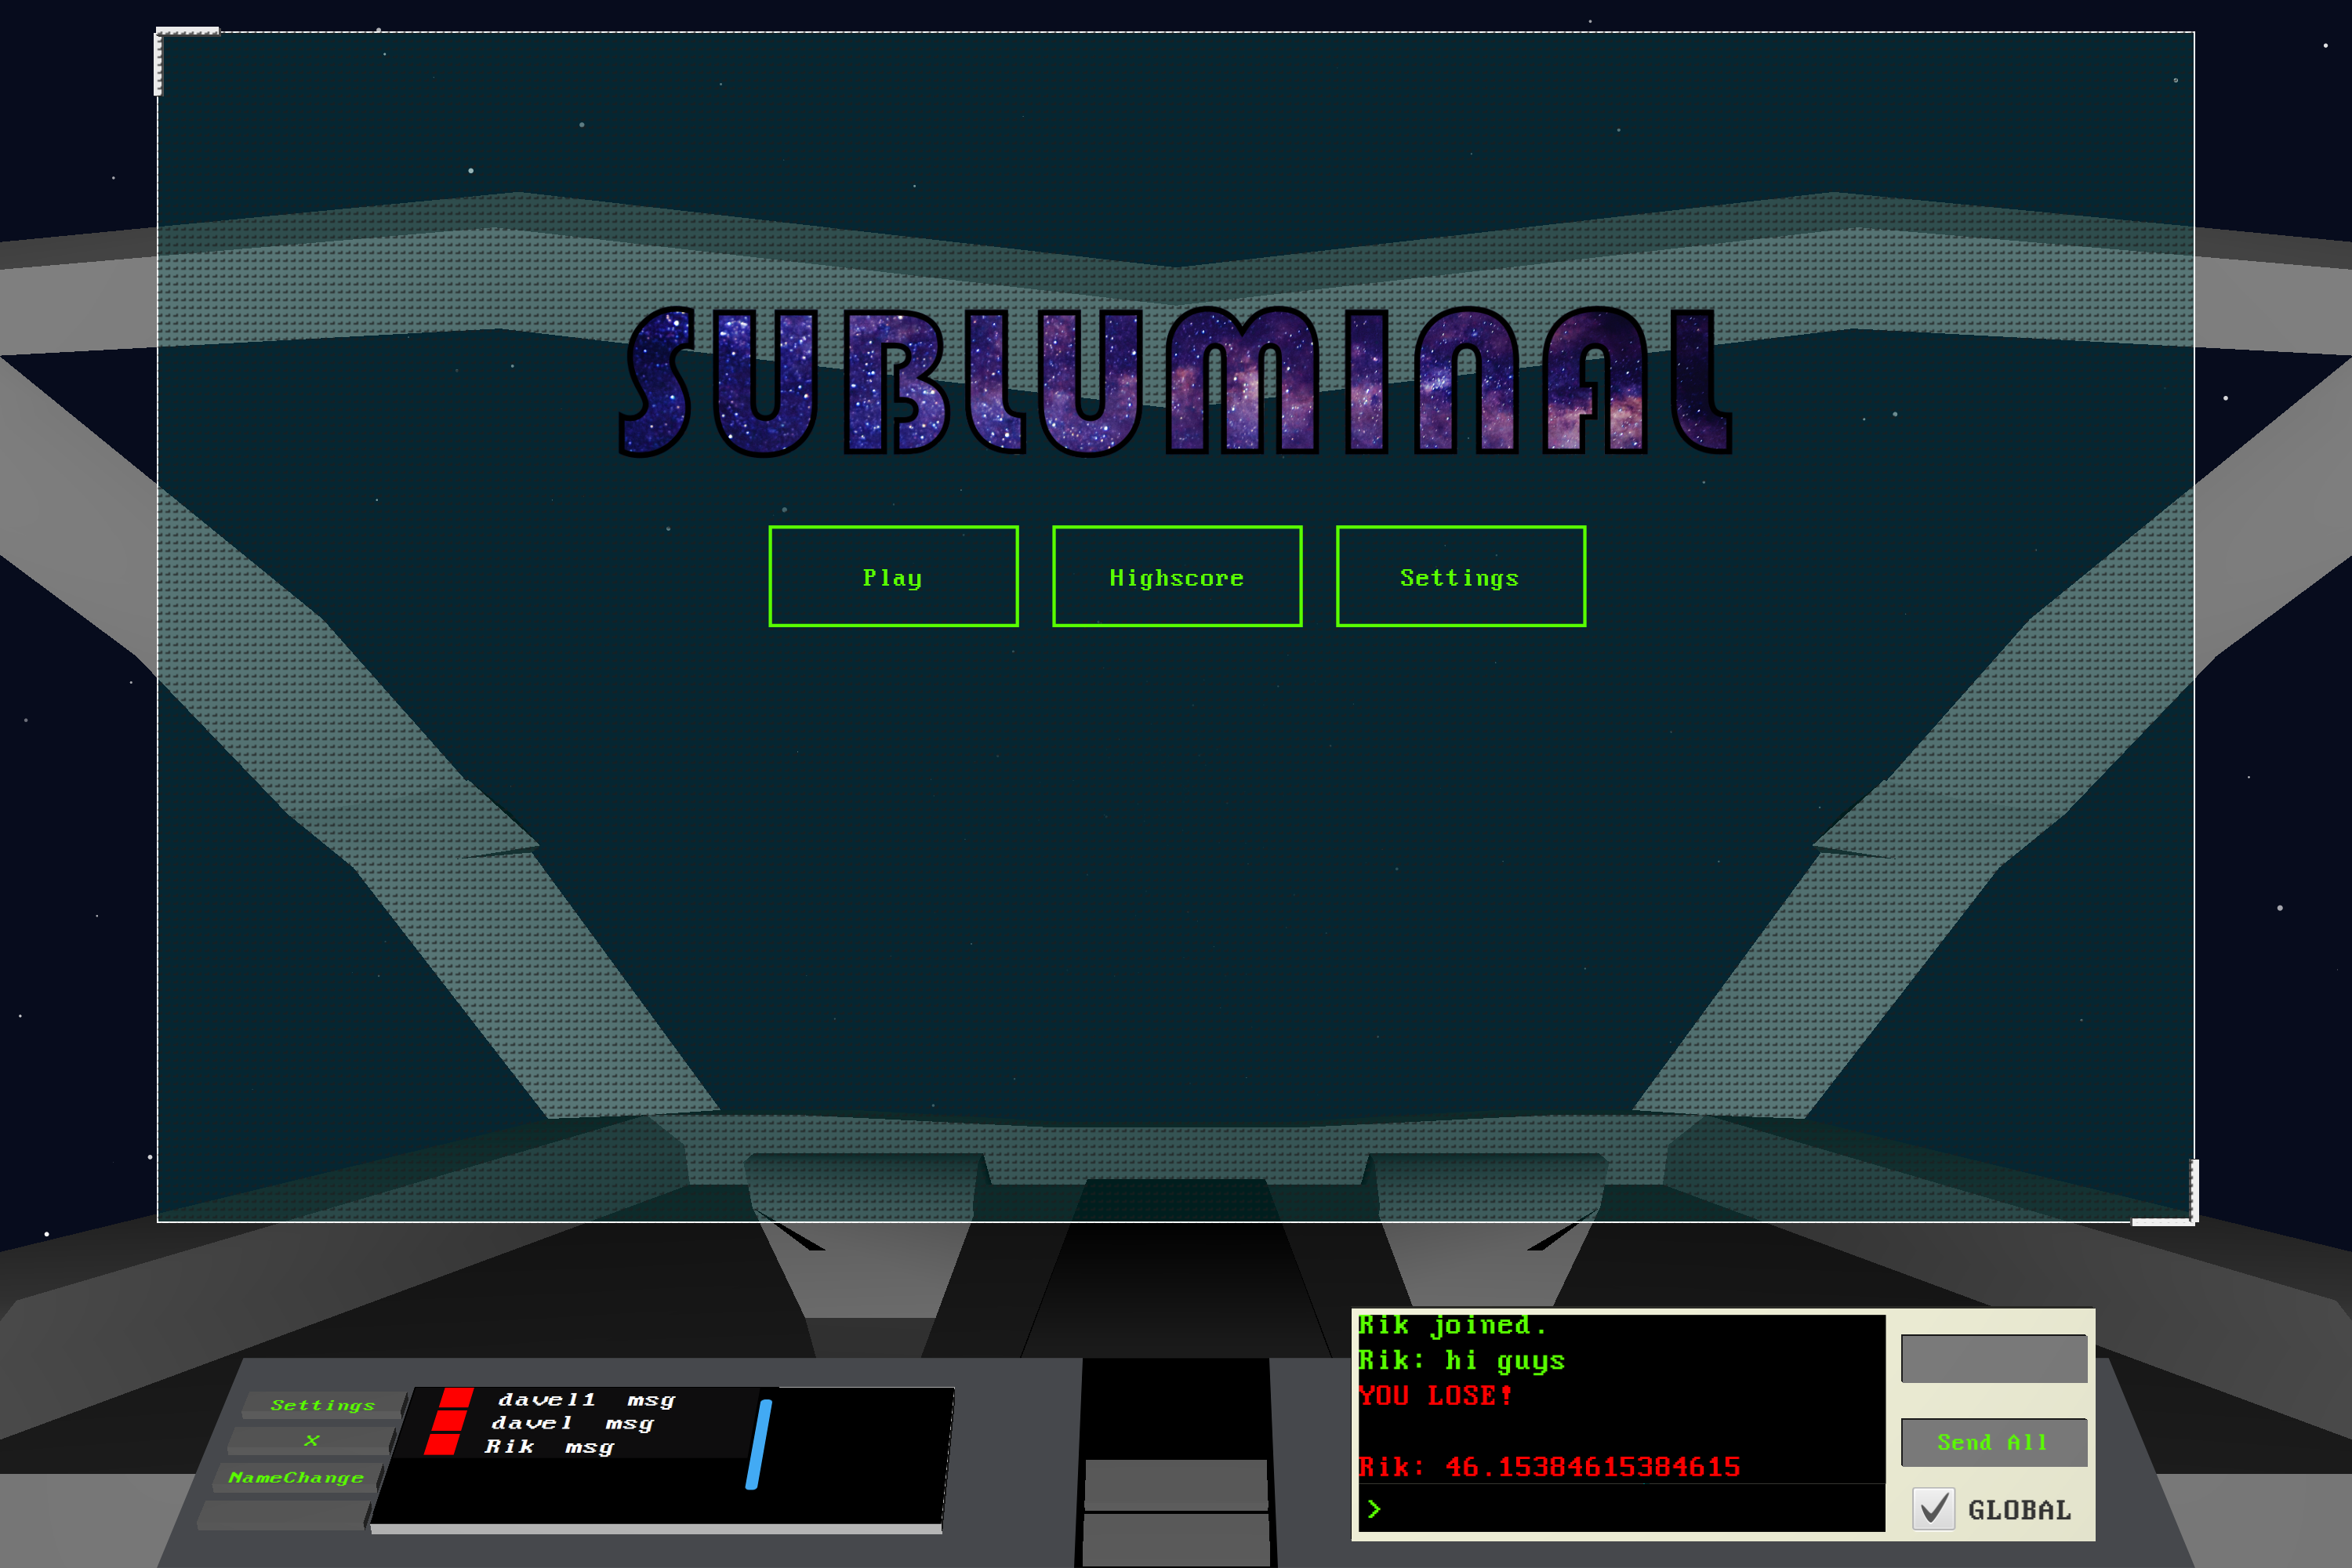
\includegraphics[width=.85\textwidth]{chapters/gamerules/menu.png}
	\caption*{Main Menu}
\end{figure}

\noindent In the bottom left of the user interface you can find buttons change your username or list all the players currently connected to the server. Pressing on \textbf{msg} next to the username starts a whisper command in the chat. Located on the bottom right is the aforementioned chat. The chat has 3 channels: global, game and whisper. Important server messages are always printed in red.\\

\noindent Going further into the play menu, you will find the lobby browser. You can use the \textbf{Refresh Lobbies} to see if somebody has already opened a game to join. If you wish to practice the game there is also in in-game tutorial waiting.

\begin{figure}[!htb]
	\centering
	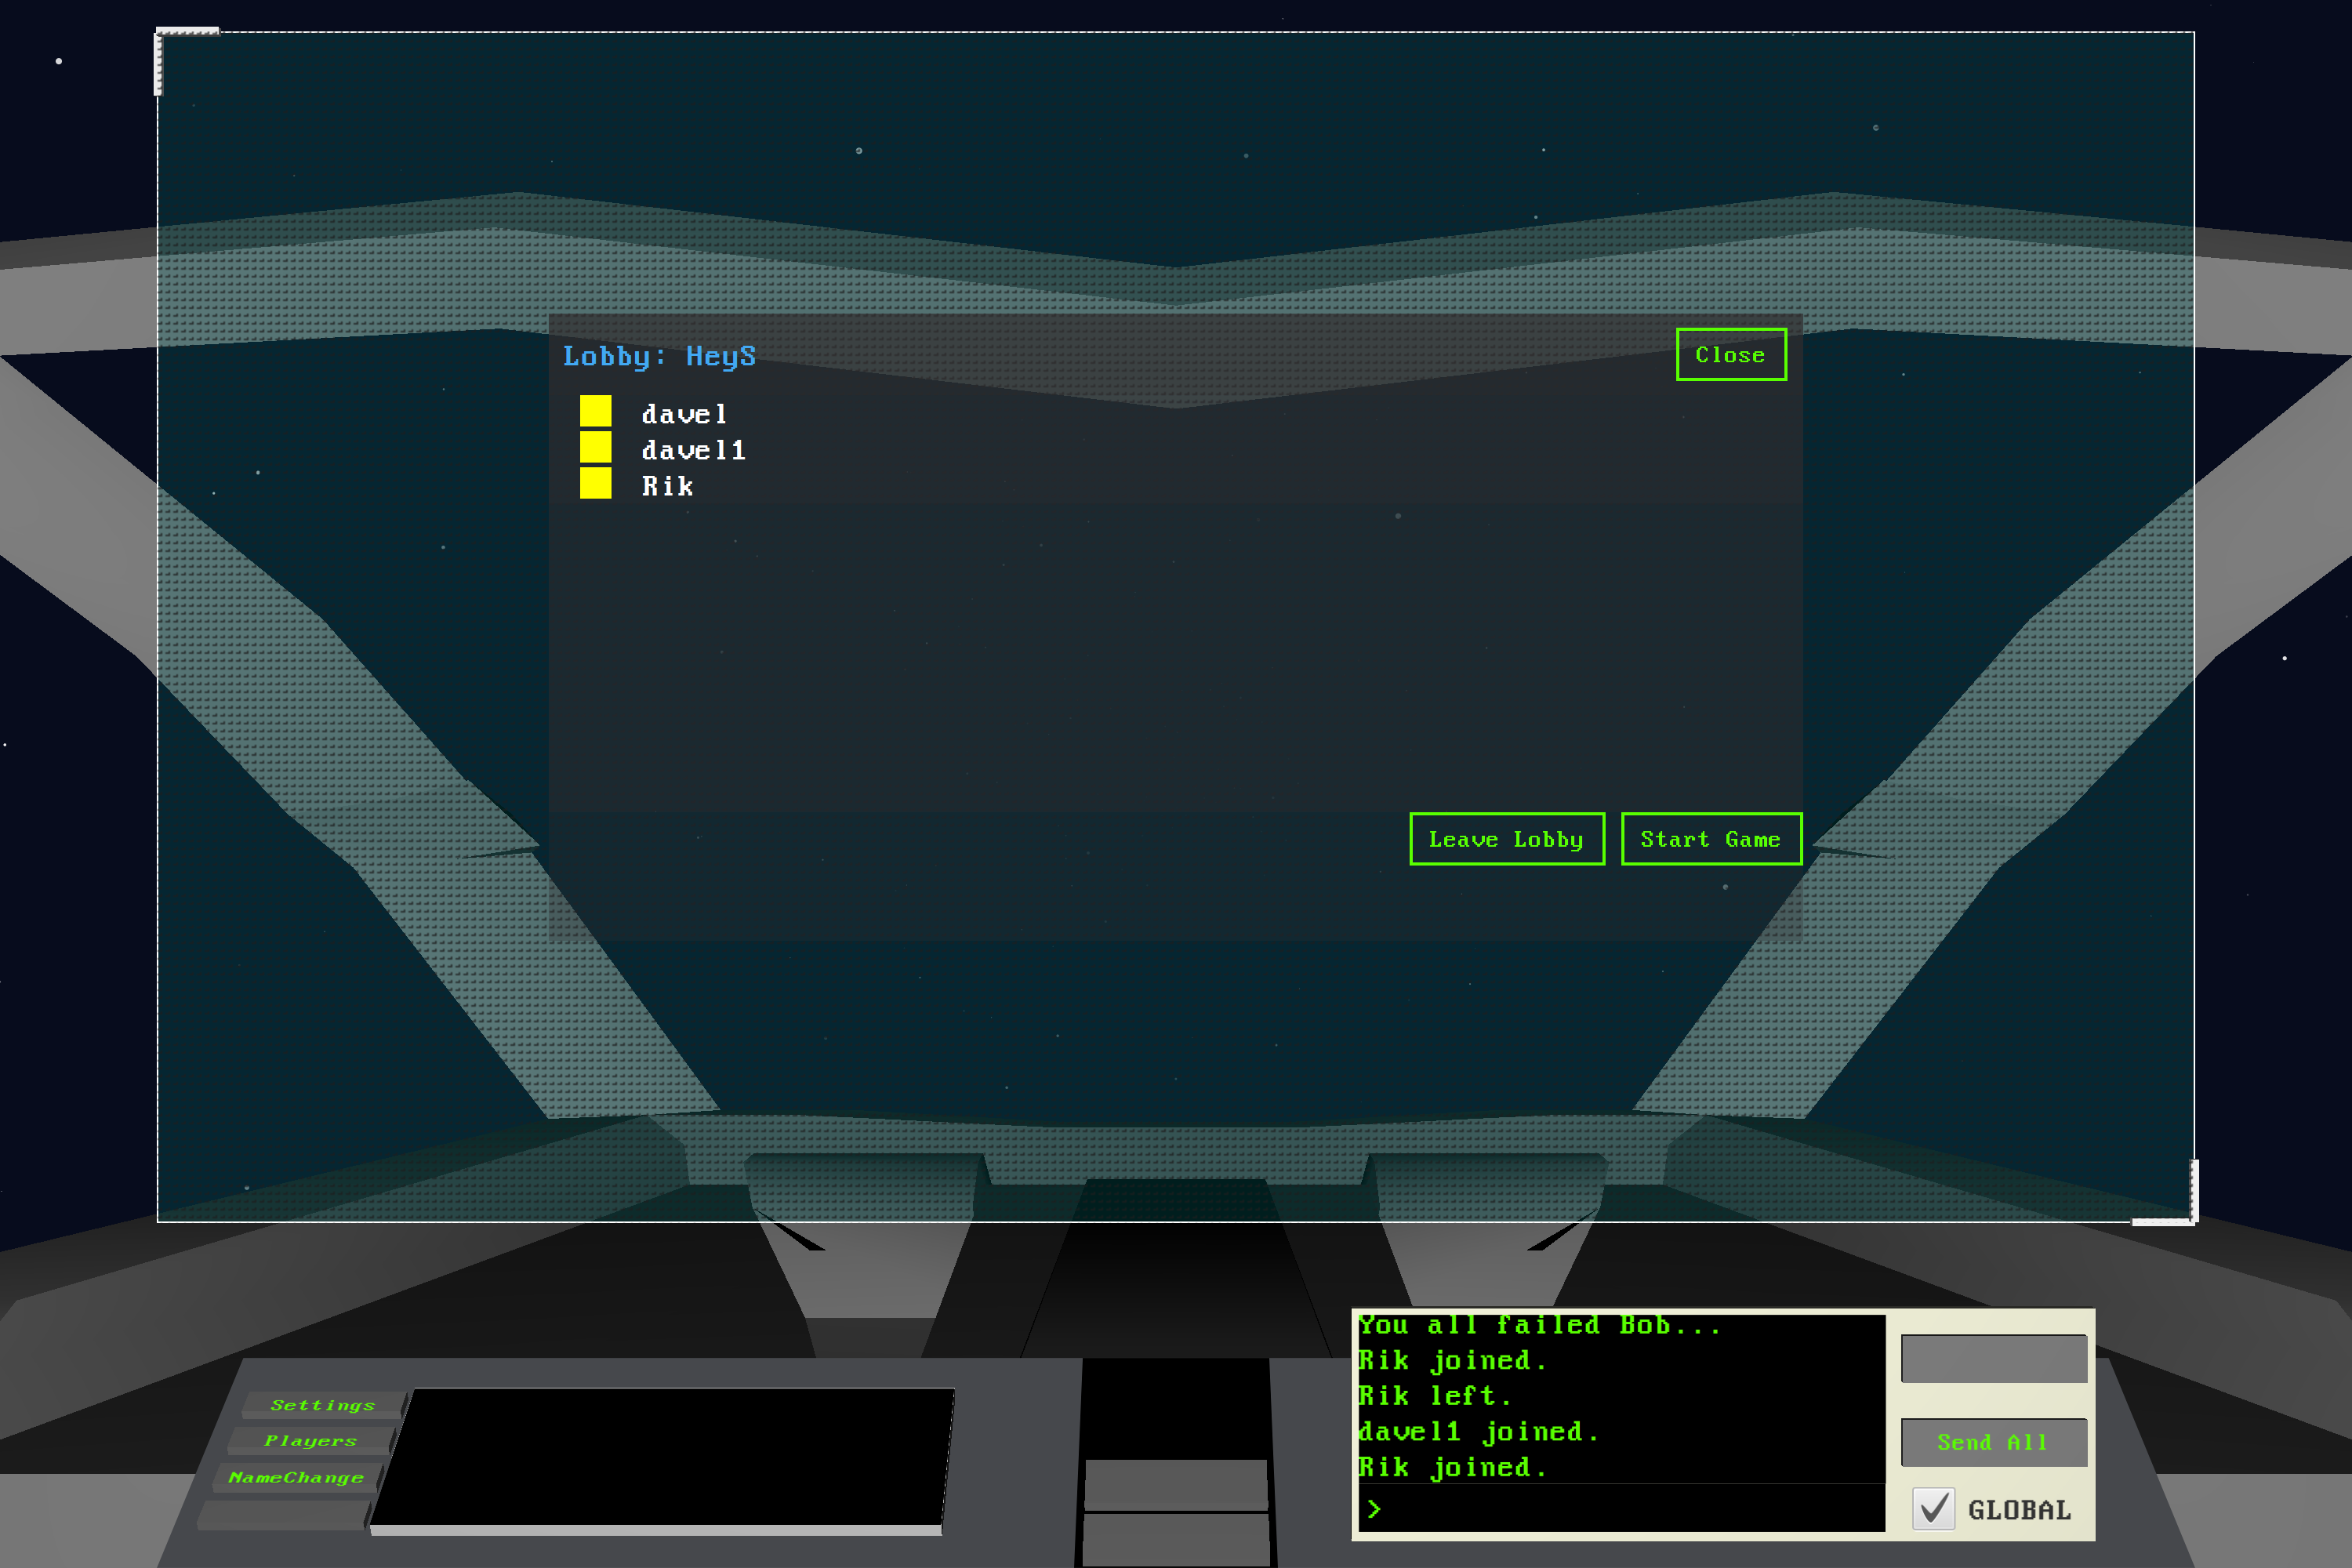
\includegraphics[width=.85\textwidth]{chapters/gamerules/lobby.png}
	\caption*{Lobby browser}
\end{figure}

\noindent Every games listed in the lobby browser has a color code. The meanings is as follows: \textbf{green}: open to join, \textbf{red}: game in progress (spectating possible) and \textbf{grey}: archived game. If there is no open lobby, you need to create one. Use the \textbf{Create Lobby} button and supply a name. Wait for other players to join then start the game. Remember: Because you created the lobby, only you can start the game.

\section*{play}
After starting the game when the map has loaded, you are presented with the view of all the stars and the starting positions of all the players. Your home star is marked with a big arrow. This is also where your mothership is first located. You want to protect it at all cast, once it is gone you loose the game. 

As you can see your home star already started producing fleet ships. You want to send them to neighbouring stars to spread your influence. You do this by Left-Clicking on two stars. The pathfinding will automatically highlight the shortes path from start to destination. Now the menu in the middle of the console activates. Input the number of fleet ships to send or send the mothership to the selected star. Once they arive, they will start to capture the star, which in turn will produce new fleet ships for you.
\begin{figure}[!ht]
	\centering
	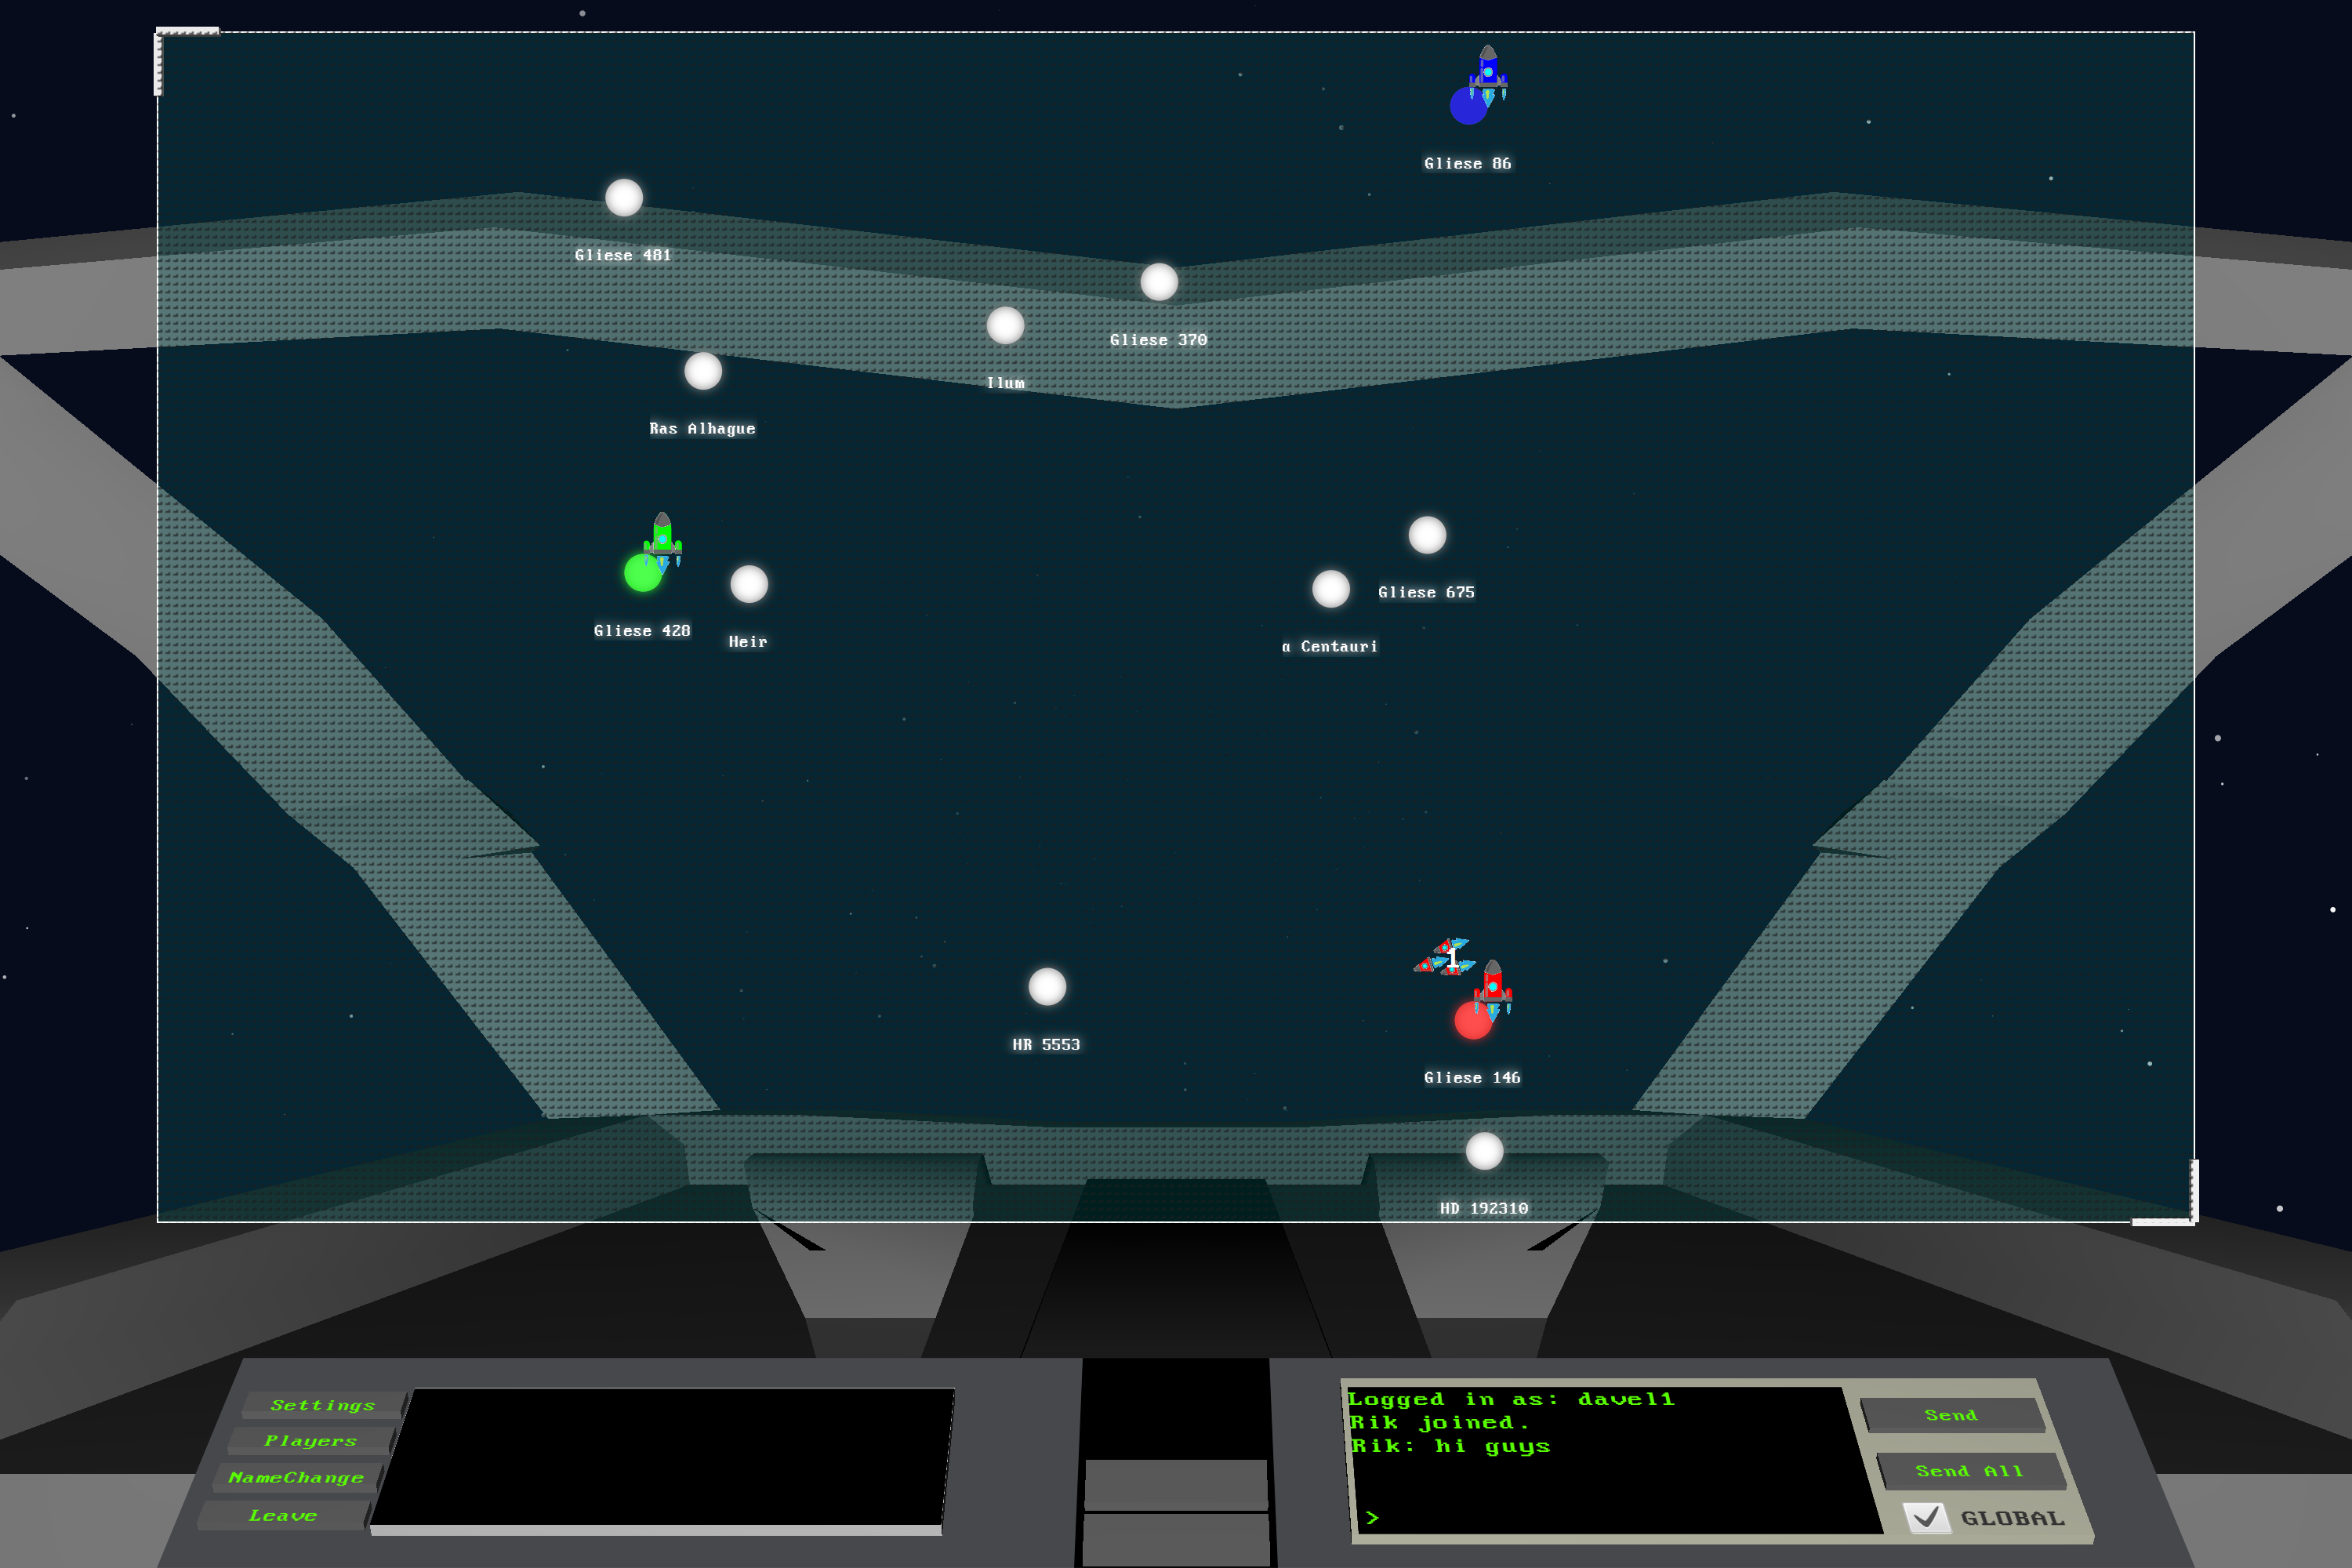
\includegraphics[width=.85\textwidth]{chapters/gamerules/gamestart.png}
	\caption*{A new game of Subluminal}
\end{figure}

You win a game by overpowering all other motherships with your fleet. When you have won a game your name will be put in the highscore list for all other players to see.

\begin{figure}[!ht]
	\centering
	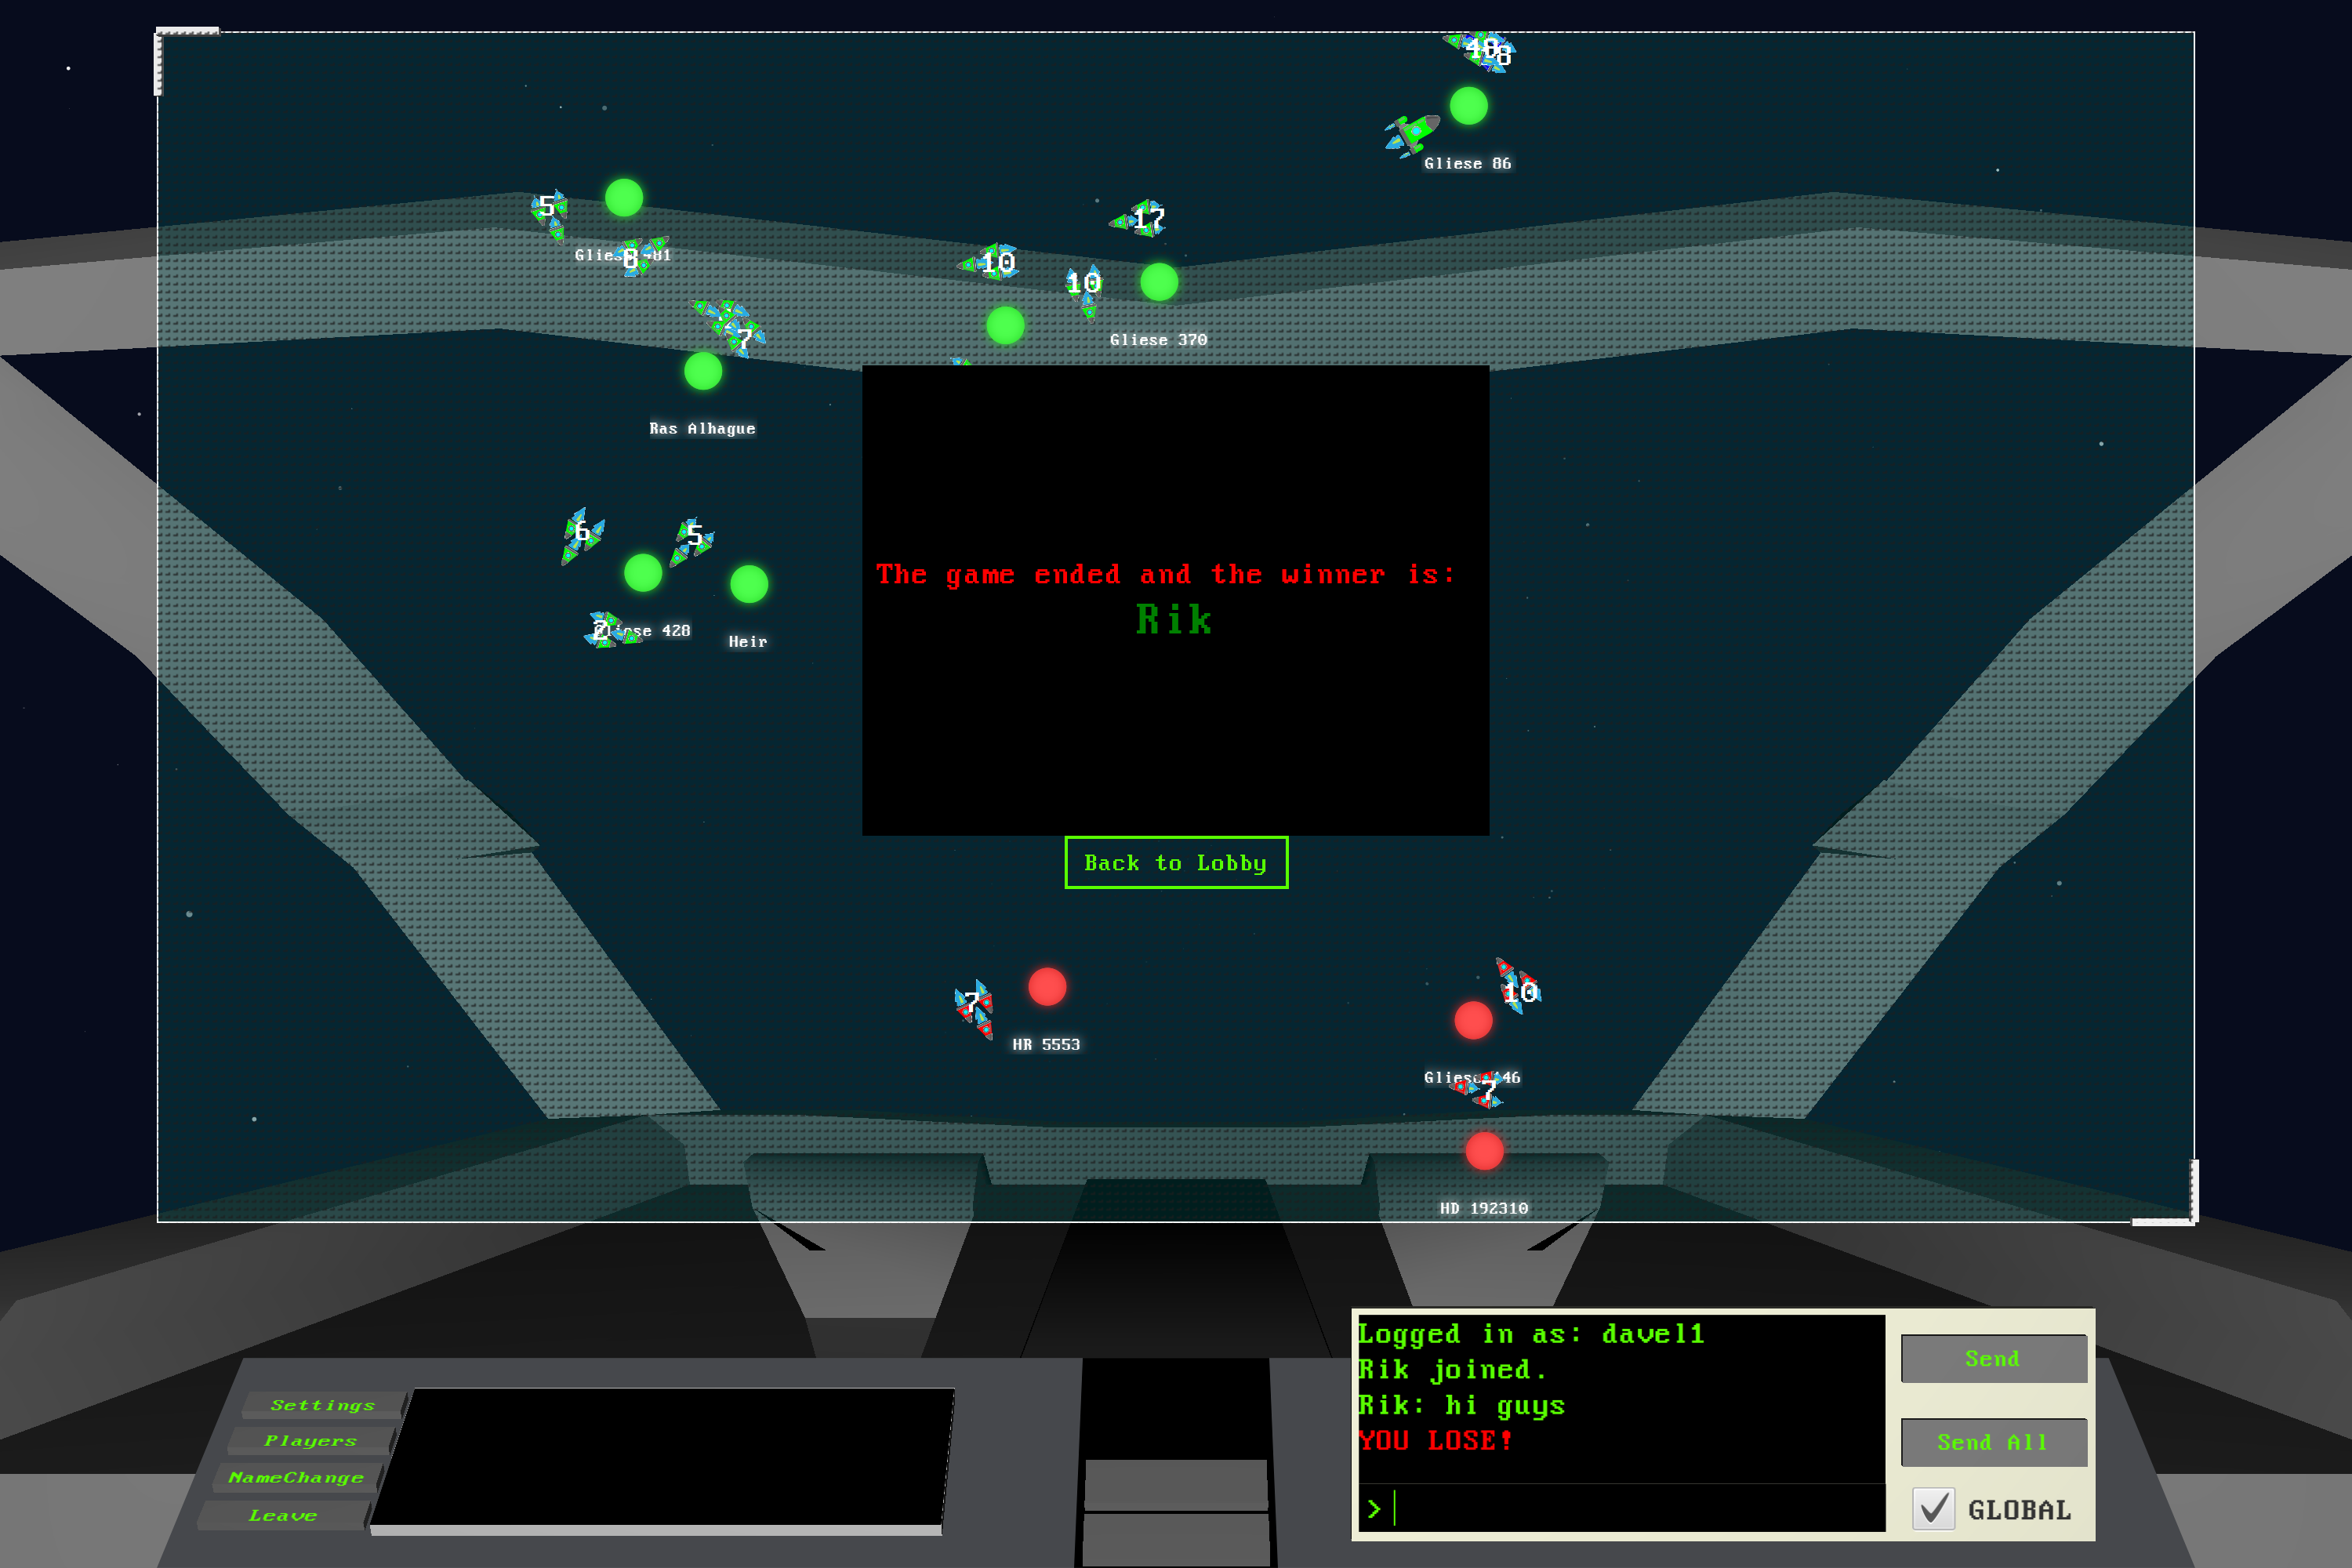
\includegraphics[width=.85\textwidth]{chapters/gamerules/gameend.png}
	\caption*{Winning Screen}
\end{figure}

\clearpage
\section*{rules}
Below you can find the basic game rules which are implemented in the game logic.

\begin{enumerate}
	\item The maximum number of players is 8.
	\item At the beginning of a game, the map is created randomly.
	\item The map consists of stars.
	\item At the beginning of a game, every player's mothership is randomly assigned to a star.
	\item You lose the game when your mothership dies.
	\item You win the game when your mothership is the only remaining mothership on the map.
	\item Every player is able to see the whole map.
	\item When a player colonizes a star, the star automatically starts to produce ships for the player, which accumulate on that star.
	\item The ships that are local to a star that is owned by a player, can be sent to neighbouring stars as fleets.
	\item Stars can be colonized by sending fleets to them. If a star already belongs to another player, dematerialization occurs between the two fleets and the winning player (the one with the bigger fleet) keeps the star.
	\item Since the fleets have to fuel up at some point, the maximum jumping distance between two stars is restricted.
	\item The rule above implicates   that further destinations can only be reached by one's ships by ``hopping'' from star to star to be able to fuel up.
	\item A pathfinding algorithm computes the shortest path between the origin and target star. The target star can only be reached by that path.
	\item ``Hopping'' can occur on both neutral and owned (colonized) stars.
	\item By hopping onto a star that is owned by an opponent, the hopping player gets punished by dematerialization of a small part of his hopping fleet.
	\item Hopping and colonizing stars are two separate processes. Accidental colonization while hopping a star can not occur.
	\item Every move one’s ships make originates from the mothership. Thus, the order takes longer to get to the concerning ships, the further their base star is away from the mothership.
	\item The rule above also implies that, the further away from one's mothership something happens, the more outdated the respective information is when it arrives at a player (i.e. his mothership).
	\item When a player orders a fleet to go colonize another star, the information about the number of available regular ships is always outdated (because of the distance). So the player simply enters the maximum number of ships to be sent and, if there are not that many, all available ships are sent.
	\item Every event on the map is broadcasted to all the players and reaches a player's mothership according to the time delay caused by the distance.
	\item The mothership can also be moved from her base, it's slower than ships.
	\item The mothership is as strong as 5 ships.
	\item If the base of the mothership is intruded, the mothership is the last one to be torn down.
\end{enumerate}